\subsubsection{Eliminierung 3 bis 9 Harmonischer}


\begin{figure}[!ht]
  \begin{center}
  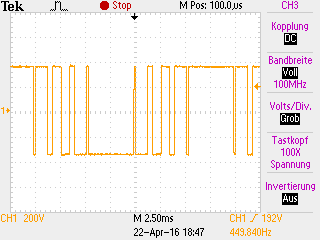
\includegraphics[width=0.48\textwidth]
  {pic/6_2_weitere_pulsmuster/6_2_1_stromform/eliminierung_3_bis_9/ALL0000/F0000TEK.png}
  \caption{$U_A (Orange)$}
  \label{fig:6_2_2_0}
  \end{center}
\end{figure}


\begin{figure}[!ht]
  \begin{center}
  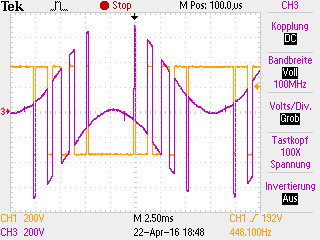
\includegraphics[width=0.48\textwidth]
  {pic/6_2_weitere_pulsmuster/6_2_1_stromform/eliminierung_3_bis_9/ALL0001/F0001TEK.png}
  \caption{$U_A (Orange), U_L (Violett)$}
  \label{fig:6_2_2_1}
  \end{center}
\end{figure}


\begin{figure}[!ht]
  \begin{center}
  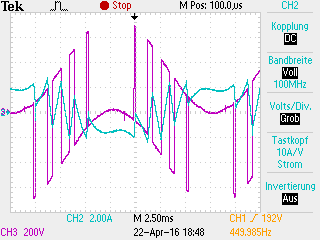
\includegraphics[width=0.48\textwidth]
  {pic/6_2_weitere_pulsmuster/6_2_1_stromform/eliminierung_3_bis_9/ALL0002/F0002TEK.png}
  \caption{$U_L (Violett), I_{L1} (Hellblau)$}
  \label{fig:6_2_2_2}
  \end{center}
\end{figure}


\clearpage